\documentclass{report}

\usepackage[utf8]{luainputenc}
\usepackage[english, russian]{babel}
\usepackage{indentfirst}
\usepackage{graphicx}
\usepackage{amsmath}
\usepackage{geometry}
\usepackage{enumitem}
\usepackage[T2A]{fontenc}
\usepackage[14pt]{extsizes}
\usepackage{listings}
\usepackage{color}

\lstset{
		language=C++,
		title=\lstname,  
		basicstyle=\footnotesize\sffamily,
		numbers=left,
		numberstyle=\scriptsize,
		tabsize=4,
		breaklines=true,
  		breakatwhitespace=true,
		keywordstyle=\color{blue}\ttfamily,
		commentstyle=\color{green}\ttfamily,   
}

\geometry{a4paper,top=2cm,bottom=2cm,left=2cm,right=1.5cm}
\setlength{\parskip}{0.5cm}
\setlist{nolistsep, itemsep=0.5cm,parsep=2pt}


\begin{document}

\begin{titlepage}

\begin{center}
\textbf{Федеральное государственное автономное образовательное учреждение высшего образования} \\
"Национальный исследовательский Нижегородский государственный университет им. Н.И. Лобачевского" (ННГУ)
\end{center}

\begin{center}
\textbf{Институт информационных технологий, математики и механики}
\end{center}

\vspace{5em}

\begin{center}
\textbf{\LARGEОТЧЕТ ПО ЛАБОРАТОРНОЙ РАБОТЕ} \\
\end{center}
\begin{center}
\textbf{\Large«Построение выпуклой оболочки для компонент бинарного изображения»} \\
\end{center}

\vspace{6em}

\newbox{\lbox}
\savebox{\lbox}{\hbox{text}}
\newlength{\maxl}
\setlength{\maxl}{\wd\lbox}
\hfill\parbox{8cm}{
\hspace*{5cm}\hspace*{-5cm}\textbf{Выполнил:} \\ Студент группы 381706-1 \\ Силенко Дмитрий Игоревич\\  \_\_\_\_\_\_\_\_ Подпись
\\ \\
\hspace*{5cm}\hspace*{-5cm}\textbf{Проверил:}\\ Доцент кафедры МОСТ, кандидат технических наук \\ \_\_\_\_\_\_\_\_ Сысоев А. В.
}

\vspace{\fill}

\begin{center} Нижний Новгород \\ 2020. \end{center}

\end{titlepage}


\setcounter{page}{2}
\tableofcontents

\newpage


\begin{center}
\section*{1. Введение}
\end{center}
\addcontentsline{toc}{section}{1. Введение}
\par \textbf{Основная цель данной работы} – реализовать алгоритм, способный выделить компоненты на бинарном изображении и далее на их основе построить выпуклую оболочку.
\par Но для начала необходимо разобраться что вообще такое бинарное изображение, как с ним можно работать, а так же что такое выпуклая оболочка.
\par \textbf{Бинарное изображение} – разновидность цифрового растрового изображения, когда каждый пиксель может представлять только один из двух цветов. Значения каждого пикселя условно кодируются как 0 и 1. Значение 0 соответствует заднему плану или фону, а 1 – переднему плану (объекту). Для нас это особенно удобно, т.к. бинарное изображение можно представить в виде двумерного массива размерностью длина изображения на его ширину, заполненного 0 и 1. Номер строчки и столбца для каждого пикселя можно интерпретировать как координаты x и y для точки в пространстве. Это, в свою очередь, позволяет применять один из известных алгоритмов для построения выпуклой оболочки набора точек. Но обо всем по порядку. 
\par \textbf{Компонентой} на изображении будем считать связанную (рассматриваем 4х связанность, т.е. проверяем окрестность пикселя только по горизонтали и вертикали) фигуру, принадлежащую объекту (состоящую из единиц). 
\begin{figure}[htbp]
  \centering
  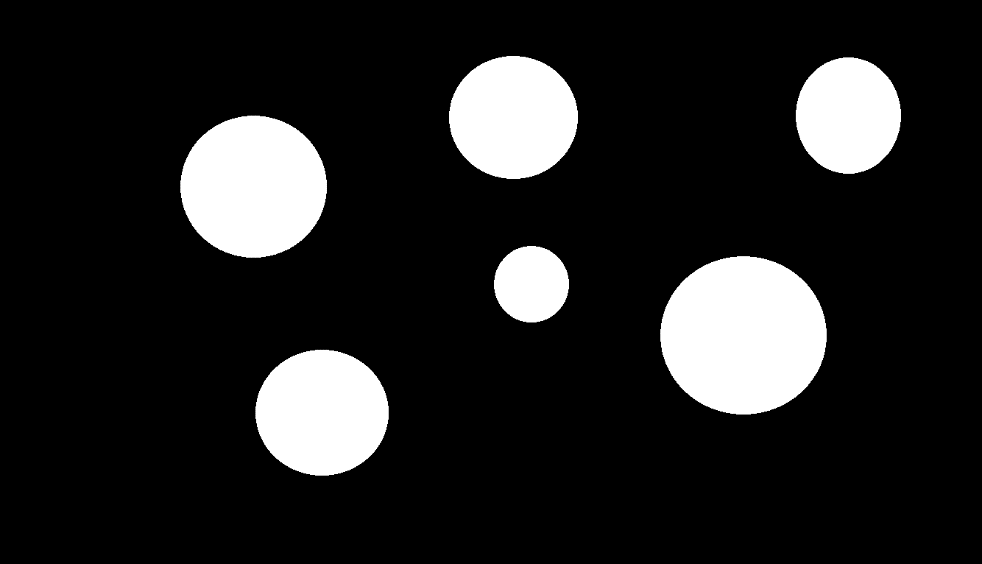
\includegraphics[width=0.8\textwidth]{../../../../modules/reports/silenko_d_convex_binary/1Binary_Image.png}
  \caption{Бинарное изображение с несколькими компонентами связанности}\label{fig:../../../../modules/reports/silenko_d_convex_binary/1Binary_Image.png}
\end{figure}
\par \textbf{Выпуклая оболочка} множества точек — такое выпуклое множество точек, что все точки фигуры также лежат в нем. Необходимо отметить, что строить мы будем не просто выпуклую оболочку, а минимальную выпуклую оболочку.
\par \textbf{Минимальная выпуклая} оболочка множества точек — это минимальная по площади выпуклая оболочка.
\begin{figure}[htbp]
  \centering
  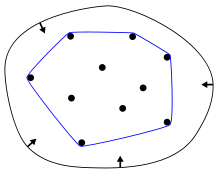
\includegraphics[width=0.4\textwidth]{../../../../modules/reports/silenko_d_convex_binary/2Convex_Hull.png}
  \caption{Выпуклая оболочка и минимальная выпуклая оболочка}\label{fig:../../../../modules/reports/silenko_d_convex_binary/2Convex_Hull.png}
\end{figure}
\par По сути, минимальная выпуклая оболочка это знакомый всем со школы выпуклый многоугольник, состоящий из точек входного множества так, что все остальные точки этого множества лежат внутри него.
 
\newpage


\begin{center}
\section*{2. Постановка задачи}
\end{center}
\addcontentsline{toc}{section}{2. Постановка задачи}
\par Для входного изображения выделить компоненты связанности, построить для них внешнюю и внутреннюю выпуклые оболочки, а так же продемонстрировать (визуализировать) результат работы программы. Полученный алгоритм необходимо распараллелить с использованием технологий OpenMP и TBB так, чтобы он корректно работал для произвольного числа процессов, работающих с исходным изображением.

\newpage


\begin{center}
\section*{3. Описание алгоритмов}
\end{center}
\addcontentsline{toc}{section}{3. Описание алгоритмов}
\subsection*{3.1 Выделение компонент на бинарном изображении}
\addcontentsline{toc}{subsection}{3.1 Выделение компонент на бинарном изображении}
\par Предположим, что исходное изображение мы перевели в бинарное и занесли значения пикселей в массив. Далее необходимо пройтись по нему и отделить компоненты друг от друга (выделить связанные области). 
\par Идея алгоритма основана на использовании уголка (маски) ABC. Проход по изображению (массиву) с ее помощью осуществляется слева направо и сверху вниз. При этом мы считаем, что за границей изображения объектов нет.
\begin{figure}[htbp]
  \centering
  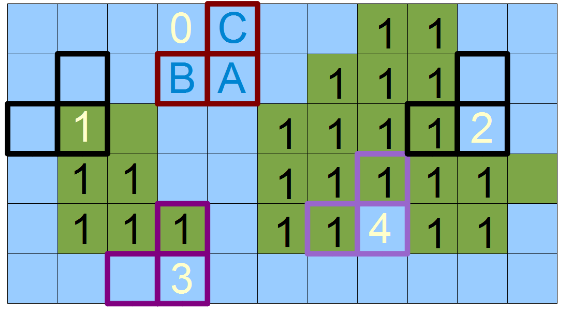
\includegraphics[width=0.6\textwidth]{../../../../modules/reports/silenko_d_convex_binary/3ABC.png}
  \caption{Маска ABC и ее возможные положения}\label{fig:../../../../modules/reports/silenko_d_convex_binary/3ABC.png}
\end{figure}
\par Рассмотрим подробнее все позиции маски:
\begin{itemize}
\item Позиция под номером 0, когда не размечен элемент A – в этом случае мы просто пропускаем пиксель
\item Позиция под номером 1, когда помечен только элемент A – можем говорить о создании нового объекта (присваиваем ему новый номер)
\item Позиция под номером 2, когда помечен элемент B (A при этом не пуст) – мы помечаем текущий пиксель A меткой, расположенной в B
\item Позиция под номером 3, когда помечен элемент C (A при этом не пуст) – мы помечаем текущий пиксель A меткой, расположенной в C
\item Позиция под номером 4, когда помечены и B и C (A при этом не пуст) – если B и C совпадают, то помечаем A так же, если не совпадают, то перенумеруем все уже обработанные пиксели помеченные как C в метку B
\end{itemize}
\begin{figure}[htbp]
  \centering
  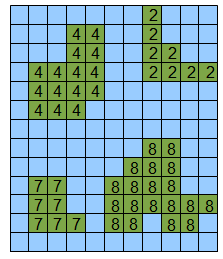
\includegraphics[width=0.4\textwidth]{../../../../modules/reports/silenko_d_convex_binary/4Get_Component.png}
  \caption{Результат выделения компонент}\label{fig:../../../../modules/reports/silenko_d_convex_binary/4Get_Component.png}
\end{figure}
\par Как видно из рисунка 4, компоненты пронумерованы непоследовательно, но для нас это и не важно. Главное, чтобы мы могли их отличать.

\subsection*{3.2 Построение внешней выпуклой оболочки с помощью прохода Джарвиса}
\addcontentsline{toc}{subsection}{3.2 Построение внешней выпуклой оболочки с помощью прохода Джарвиса}
\par Среди точек  $a_1$, ...,  $a_n$ выберем самую нижнюю (по координате y) левую (по координате x) точку $b_1$, она точно будет являться вершиной выпуклой оболочки. Теперь для каждой текущей точки $b_i$ (1 $\leq$ i $\leq$ n) ищется такая точка $b_i+_1$ (из оставшихся + самая первая), в которой будет образовываться наибольший угол между прямыми $b_i-_1$ $b_i$ и $b_i$ $b_i+_1$. Уточним, что при поиске второй точки в качестве $b_0$ берется точка с координатами ($x_1$ – 2, $y_1$) (к примеру). Найденная таким образом точка $b_i+_1$ будет следующей вершиной выпуклой оболочки. При этом нет необходимости искать сам угол. Достаточно вычислить его косинус (через скалярное произведения, используя координаты точек). При этом ищется минимальный косинус (чем он меньше, чем больше угол). Нахождение вершин продолжается до тех пор, пока $b_i+_1 \neq b_1$. Если для нескольких точек косинус одинаковый (они лежат на одной прямой), то выбирается наиболее удаленная от текущей. 
\begin{figure}[htbp]
  \centering
  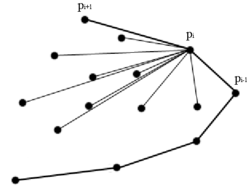
\includegraphics[width=0.4\textwidth]{../../../../modules/reports/silenko_d_convex_binary/5Jarvis.png}
  \caption{Построение выпуклой оболочки проходом Джарвиса}\label{fig:../../../../modules/reports/silenko_d_convex_binary/5Jarvis.png}
\end{figure}

\subsection*{ 3.3 Построение внутренней выпуклой оболочки}
\addcontentsline{toc}{subsection}{3.3 Построение внутренней выпуклой оболочки}
\par Внутренняя выпуклая оболочка должна соединять пиксели, принадлежащие компоненте, попавшей во внешнюю выпуклую оболочку. При этом из каждой компоненты выбирается только один пиксель.
\par Для этого при проверке ненулевых пикселей изображения заводятся два вектора: корректности и запрета. Вектор корректности будет проверять, есть ли компонента, которой принадлежит текущий пиксель во внешней выпуклой оболочке, а вектор запрета – брали ли уже из этой компоненты пиксели. Итак, для каждого пикселя проверяется есть ли его компонента в векторе корректности. Если нет, то пиксель просто пропускается. Если есть и при этом его компоненты нет в векторе запрета, то пиксель добавляется в внутреннюю выпуклую оболочку, а его компонента – в вектор запрета. Если же пиксель есть и в векторе корректности и в векторе запрета, то он также пропускается.
\begin{figure}[htbp]
  \centering
  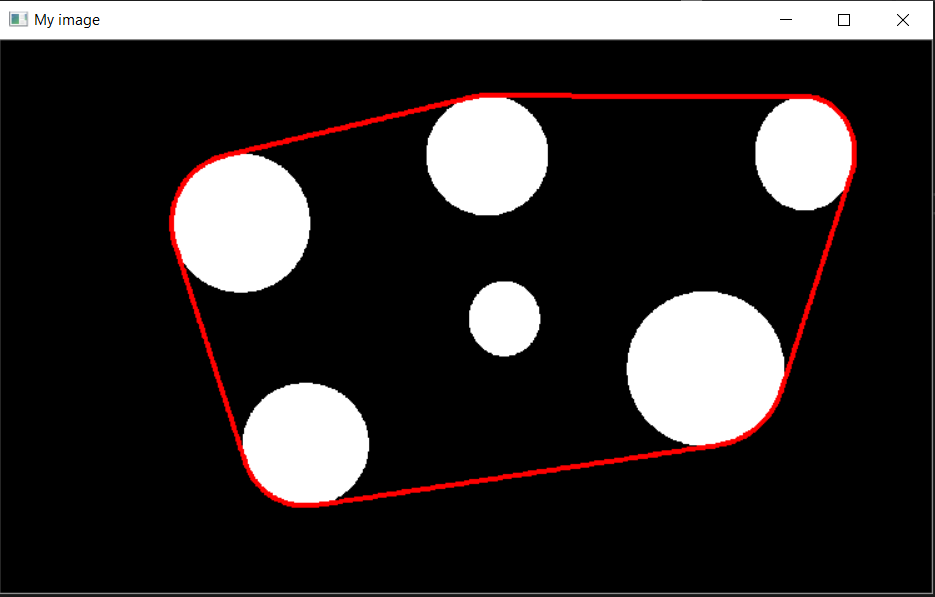
\includegraphics[width=0.6\textwidth]{../../../../modules/reports/silenko_d_convex_binary/6Outside.png}
  \caption{Внешняя выпуклая оболочка}\label{fig:../../../../modules/reports/silenko_d_convex_binary/6Outside.png}
\end{figure}
\begin{figure}[htbp]
  \centering
  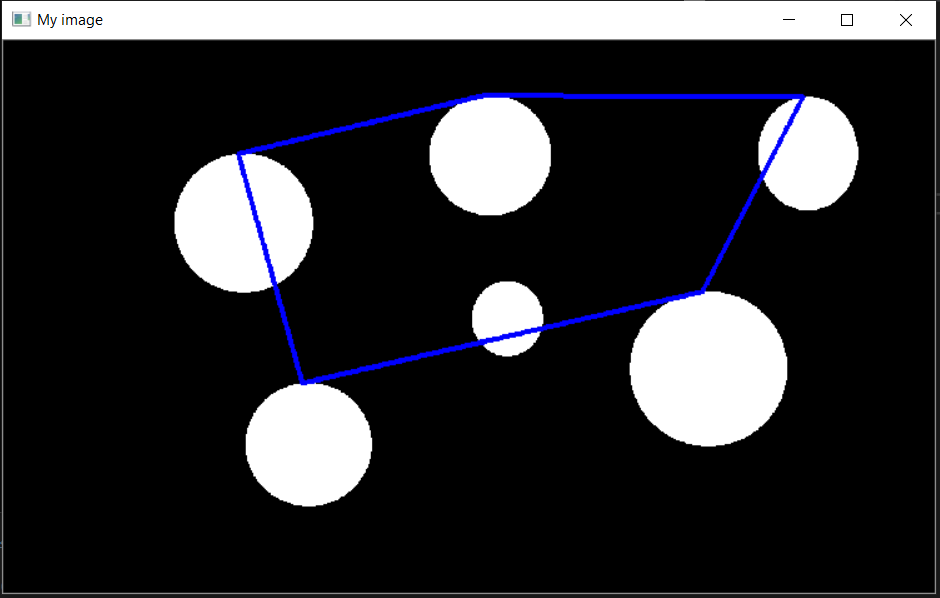
\includegraphics[width=0.6\textwidth]{../../../../modules/reports/silenko_d_convex_binary/7Inside.png}
  \caption{Соответствующая ей внутренняя выпуклая оболочка}\label{fig:../../../../modules/reports/silenko_d_convex_binary/7Inside.png}
\end{figure}
\par На рисунках 6 и 7 можно увидеть результат выделения как внешней, так и внутренней выпуклых оболочек

\newpage


\begin{center}
\section*{4. Схема распараллеливания}
\end{center}
\addcontentsline{toc}{section}{4. Схема распараллеливания}
\par Из описания алгоритма выделения компонент можно увидеть, что при не совпадении значений в элементах B и C возникает необходимость изменения в уже пройденной части изображения или массива. Таких вызовов, как правило, достаточно много из-за чего они занимают существенное время. Поэтому именно эта часть и подвергается распараллеливанию с использованием обеих технологий. Принцип у них одинаковый: строчки матрицы (изображения) от начальной до текущей делятся между процессами, те находят в них пиксели, помеченные как C, и помечают их как B. Соответственно, в версии OpenMP это реализовано при помощи дерективы \#pragma omp for. В версии TBB – tbb::parallel\_for с использованием лямбда-выражения в качестве замены объявлению класса функтора.

\newpage


\begin{center}
\section*{5. Описание программной реализации}
\end{center}
\addcontentsline{toc}{section}{5. Описание программной реализации}
\par В программе имеется три основных модуля: silenko\_d\_convex\_binary\_seq, silenko\_d\_convex\_binary\_omp и silenko\_d\_convex\_binary\_tbb. В первом из них реализована исключительно последовательная версия алгоритма, в то время как во втором и в третьем, помимо последовательной, присутствуют так же omp- и tbb-версии. Пройдем сначала по методам, присутствующих во всех этих модулях. В первую очередь это случайная генерация массива заданного размера из 0 и 1 (getRandomMas), как альтернатива загрузке реального изображения. Далее, последовательная версия выделения компонент на изображении (функция getComponent). В первом модуле она является основной, а во втором и третьем необходима для сравнения времени работы с ее параллельным аналогом. После этого необходимо найти внешнюю выпуклую оболочку (метод Jarvis и два вспомогательных – length для определения расстояния до точки и cosvec для вычисления косинуса между векторами). И наконец, нахождение внутренней выпуклой оболочки при помощи функции Inside.
\par Что же касается второго и третьего модуля, то в них  присутствуют методы getComponent\_OMP и getComponent\_TBB соответственно, для нахождения компонент связанности с использованием нескольких потоков.

\newpage


\begin{center}
\section*{6. Подтверждение корректности}
\end{center}
\addcontentsline{toc}{section}{6. Подтверждение корректности}
\par Для подтверждения корректности работы программы были написаны 5 тестов с использованием библиотеки для модульного тестирования Google Testing Framework. 3 из них проверяют правильность работы при нестандартном размещении точек: когда они находятся на одной прямой, когда они размещены по сторонам одного прямоугольника и когда точка вообще одна. Еще один тест проверяет правильность построения внутренней выпуклой оболочки при таком расположении точек, что ответ известен заранее. Последний же отличается в зависимости от модуля. В последовательной версии он просто проверяет корректность вычисления и внутренней и внешней выпуклой оболочки. В версиях OpenMP и TBB последовательная версия сравнивается с соответствующей параллельной. При этом происходит замер времени работы для оценки качества эффективности работы параллельных версий. Все тесты проходятся успешно, что и является подтверждением корректности.

\newpage


\begin{center}
\section*{7. Эксперименты}
\end{center}
\addcontentsline{toc}{section}{7. Эксперименты}
\par Эксперименты проводились на ПК с следующими параметрами:

\begin{itemize}
\item Операционная система: Windows 10 Домашняя
\item Процессор: Intel(R) Core™ i5-8250U CPU @ 1.60 GHz
\item Оперативная память: 4 Gb
\item Версия Visual Studio: 2017
\end{itemize}

\par В таблице 1 приведена зависимость времени работы алгоритма при разном числе потоков. 
\par Размер матрицы: 1000x1000.

\begin{table}[!h]
\caption{Время работы алгоритма в зависимости от числа потоков.}
\centering
\begin{tabular}{|c|c|c|c|c|c|}
\hline
	{\begin{tabular}[c]{@{}c@{}}Количество\\ потоков\end{tabular}} & 
	{\begin{tabular}[c]{@{}c@{}}Время работы\\последовательного\\ алгоритма\end{tabular}} & 
	{\begin{tabular}[c]{@{}c@{}}Время\\работы\\OpenMP\end{tabular}} & 
	{\begin{tabular}[c]{@{}c@{}}Время\\работы\\TBB\end{tabular}} & 
	{\begin{tabular}[c]{@{}c@{}}Ускорение\\OpenMP\end{tabular}} & 
	{\begin{tabular}[c]{@{}c@{}}Ускорение\\TBB\end{tabular}} 
\\ \cline{1-6}

1	& 27.24	    & 32.0891		& 32.7382		& 0.84888		& 0.83511		\\ \hline
2   & 27.0054     & 16.747       	& 17.5076        	& 1.61255		& 1.54249           \\ \hline
4   & 27.1356     & 10.0512       	& 10.4043         	& 2.69973		& 2.60811          \\ \hline
\end{tabular}
\end{table}

\par Исходя из этой таблицы можно сделать вывод, что программа работает эффективно, с ростом числа потоков время работы уменьшается. Отдельно стоит отметить, что растет оно не так быстро, как, возможно, ожидалось. Это можно объяснить. Распараллелен не весь алгоритм выделения компонент на изображении, а только его часть, что не позволяет получить максимальное ускорение. И тем не менее, оно велико, благодаря тому, что распараллеленная часть вызывается достаточно часто и на все растущих данных. На одном процессе обе параллельные версии работают медленнее, чем последовательная, в следствии накладных расходов на создание потока и инициализацию необходимых данных. В остальном же время работы как TBB, так и OpenMP версии сопоставимы. Они обе дают вполне неплохое ускорение. TBB работает чуть медленнее в силу использования лямбда-выражения, которое, в отличие от класса, при каждом новом заходе в него (а таких много) заново инициализирует нужные данные. Зато благодаря этому объем кода сократился многократно, а его понятность и простота даже выросли.

\newpage


\begin{center}
\section*{8. Заключение}
\end{center}
\addcontentsline{toc}{section}{7. Заключение}
\par Эта лабораторная работа позволила мне лучше понять алгоритм выделения компонент на бинарном изображении, как можно иначе интерпретировать это изображение, а также познакомится с новым алгоритмом построения выпуклой оболочки – алгоритмом Джарвиса.
\par В данной работе мне удалось реализовать все необходимые алгоритмы для построения выпуклой оболочки для компонент бинарного изображения. Кроме того, алгоритм выделения компонент удалось успешно распараллелить с использованием двух технологий – OpenMP и TBB. В качестве подтверждения правильности работы алгоритмов были написаны тесты, которые успешно проходятся.

\newpage


\begin{thebibliography}{9}
\addcontentsline{toc}{section}{Литература}
\bibitem{Habr} Сообщество IT-специалистов Habr. Подсчет числа объектов на бинарном изображении: 
https://habr.com/ru/post/119244/
\bibitem{Wikipedia1} Википедия: свободная электронная энциклопедия на русском языке:
https://ru.wikipedia.org/wiki/Бинарное\_изображение
\bibitem{Wikipedia2} Википедия: свободная электронная энциклопедия на русском языке:
https://ru.wikipedia.org/wiki/Алгоритм\_Джарвиса 
\end{thebibliography}
\newpage


\begin{center}
\section*{Приложение}
\end{center}
\addcontentsline{toc}{section}{Приложение}
\lstinputlisting[language=C++]{../../../../modules/task_1/silenko_d_convex_binary/convex_binary.h}
\lstinputlisting[language=C++]{../../../../modules/task_1/silenko_d_convex_binary/convex_binary.cpp}
\lstinputlisting[language=C++]{../../../../modules/task_1/silenko_d_convex_binary/main.cpp}

\lstinputlisting[language=C++]{../../../../modules/task_2/silenko_d_convex_binary_omp/convex_binary_omp.h}
\lstinputlisting[language=C++]{../../../../modules/task_2/silenko_d_convex_binary_omp/convex_binary_omp.cpp}
\lstinputlisting[language=C++]{../../../../modules/task_2/silenko_d_convex_binary_omp/main.cpp}

\lstinputlisting[language=C++]{../../../../modules/task_3/silenko_d_convex_binary_tbb/convex_binary_tbb.h}
\lstinputlisting[language=C++]{../../../../modules/task_3/silenko_d_convex_binary_tbb/convex_binary_tbb.cpp}
\lstinputlisting[language=C++]{../../../../modules/task_3/silenko_d_convex_binary_tbb/main.cpp}

\end{document}